\documentclass[12pt]{article}
\usepackage[utf8]{inputenc}
\usepackage[spanish]{babel}
\usepackage{amsmath, amssymb}
\usepackage{graphicx}
\usepackage{geometry}
\usepackage{booktabs}

\geometry{a4paper, margin=2.5cm}

\title{Tarea 10}
\author{David Stiven Muñoz Amaya -- 20202020071}
\date{}

\begin{document}

\begin{center}
    {\LARGE \textbf{Tarea 10}}\\[0.3em]
    {\large David Stiven Muñoz Amaya -- 20202020071}
\end{center}
\vspace{0.5em}

\section*{Erlang C ($M/M/k$)}

\subsection*{1. Diagrama de transición de estados}

\begin{figure}[h!]
    \centering
    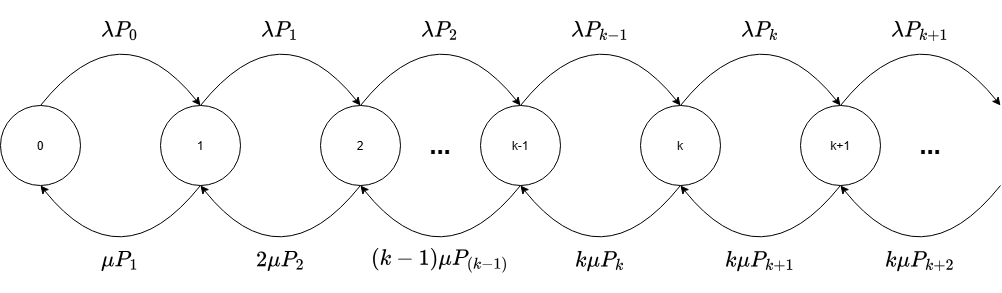
\includegraphics[width=0.75\textwidth]{Erlang_C_Diagram.drawio.png}
    \caption{Diagrama de transición de estados para el modelo Erlang C.}
    \label{fig:diagrama_transicion}
\end{figure}

\subsection*{2. Ecuaciones de estado estacionario}

\begin{table}[h!]
\centering
\renewcommand{\arraystretch}{1.4}
\resizebox{\textwidth}{!}{%
\begin{tabular}{@{}cccccc@{}}
\toprule
\textbf{Estado} & \textbf{Tasa promedio de salida del estado} & $=$ & \textbf{Tasa promedio de llegada al estado} & & \textbf{Probabilidades} \\ 
\midrule
$0$ & $\lambda P_0$ & $=$ & $\mu P_1$ & $\implies$ & $P_1 = \dfrac{\lambda}{\mu} P_0$ \\
$1$ & $\mu P_1 + \lambda P_1$ & $=$ & $2\mu P_2 + \lambda P_0$ & $\implies$ & $P_2 = \dfrac{\lambda}{2\mu} P_1$ \\
$2$ & $\lambda P_2 + 2\mu P_2$ & $=$ & $\lambda P_1 + (k-1)\mu P_{k-1}$ & $\implies$ & $P_{k-1} = \dfrac{\lambda}{(k-1)\mu} P_2$ \\
$k-1$ & $\lambda P_{k-1} + (k-1)\mu P_{k-1}$ & $=$ & $\lambda P_{2} + k\mu P_k$ & $\implies$ & $P_{k} = \dfrac{\lambda}{k\mu} P_{k-1}$ \\
$k$ & $\lambda P_k + k\mu P_k$ & $=$ & $\lambda P_{k-1} + k\mu P_{k+1}$ & $\implies$ & $P_{k+1} = \dfrac{\lambda}{k\mu} P_k$ \\
$k+1$ & $\lambda P_{k+1} + k\mu P_{k+1}$ & $=$ & $\lambda P_k + k\mu P_{k+2}$ & $\implies$ & $P_{k+2} = \dfrac{\lambda}{k\mu} P_{k+1}$ \\
\bottomrule
\end{tabular}%
}
\end{table}

\subsection*{3. Calcular $P_n$ en función de $P_0$}

Para los primeros estados se tiene la relación general:
\[
P_n = \frac{1}{n!} \left( \frac{\lambda}{\mu} \right)^n P_0
\]

Como a partir de $k$ servidores la tasa ya no aumenta sino que queda fija en $k\mu$, se analiza en 2 casos (donde $n-k$ representa la distancia que hay entre $k$ y $n$):

\[
P_n = 
\begin{cases} 
\displaystyle \frac{1}{n!} \left( \frac{\lambda}{\mu} \right)^n P_0, & \text{si } 0 \le n < k \\[1.5em]
\displaystyle \frac{1}{k! \, k^{n-k}} \left( \frac{\lambda}{\mu} \right)^n P_0, & \text{si } n \ge k 
\end{cases}
\]

\subsection*{4. $P_n$ en función de los parámetros $\lambda$ y $\mu$}

Por condición de normalización:
\[
P_0 + P_1 + P_2 + \dots = 1 \implies \sum_{n=0}^{\infty} P_n = 1
\]

Separando la sumatoria en los dos casos:
\[
\sum_{n=0}^{k-1} P_n + \sum_{n=k}^{\infty} P_n = 1
\]

Sustituyendo las expresiones de $P_n$ en función de $P_0$:
\[
\sum_{n=0}^{k-1} \left[ \frac{1}{n!} \left( \frac{\lambda}{\mu} \right)^n P_0 \right] + \sum_{n=k}^{\infty} \left[ \frac{1}{k! \, k^{n-k}} \left( \frac{\lambda}{\mu} \right)^n P_0 \right] = 1
\]

Factorizando $P_0$:
\[
P_0 \left( \sum_{n=0}^{k-1} \frac{1}{n!} \left( \frac{\lambda}{\mu} \right)^n + \sum_{n=k}^{\infty} \frac{1}{k! \, k^{n-k}} \left( \frac{\lambda}{\mu} \right)^n \right) = 1
\]

Desarrollando la segunda sumatoria:
\[
\sum_{n=k}^{\infty} \frac{1}{k! \, k^{n-k}} \left( \frac{\lambda}{\mu} \right)^n = \frac{1}{k!} \left( \frac{\lambda}{\mu} \right)^k \sum_{n=k}^{\infty} \left( \frac{\lambda}{k\mu} \right)^{n-k}
\]

Haciendo el cambio de variable $m = n - k$ (cuando $n = k \to m = 0$):
\[
= \frac{1}{k!} \left( \frac{\lambda}{\mu} \right)^k \sum_{m=0}^{\infty} \left( \frac{\lambda}{k\mu} \right)^m
\]

Definiendo $A = \frac{\lambda}{k\mu}$, dado que $|A| < 1$ (para que la serie geométrica converja, es decir, $\lambda < k\mu$):

\[
\sum_{m=0}^{\infty} A^m = \frac{1}{1 - A} = \frac{1}{1 - \frac{\lambda}{k\mu}} = \frac{k\mu}{k\mu - \lambda}
\]

Por lo tanto, el segundo término resulta en:
\[
= \frac{1}{k!} \left( \frac{\lambda}{\mu} \right)^k \left( \frac{k\mu}{k\mu - \lambda} \right)
\]

Sustituyendo en la ecuación con $P_0$ factorizado y despejando $P_0$:
\[
P_0 = \left[ \sum_{n=0}^{k-1} \frac{1}{n!} \left( \frac{\lambda}{\mu} \right)^n + \frac{1}{k!} \left( \frac{\lambda}{\mu} \right)^k \left( \frac{k\mu}{k\mu - \lambda} \right) \right]^{-1}
\]

Finalmente, reemplazando $P_0$ en la expresión por partes de $P_n$:

\[
P_n = 
\begin{cases} 
\displaystyle \frac{1}{n!} \left( \frac{\lambda}{\mu} \right)^n \left[ \sum_{i=0}^{k-1} \frac{1}{i!} \left( \frac{\lambda}{\mu} \right)^i + \frac{1}{k!} \left( \frac{\lambda}{\mu} \right)^k \left( \frac{k\mu}{k\mu - \lambda} \right) \right]^{-1}, & \text{si } 0 \le n < k \\[2em]
\displaystyle \frac{1}{k! \, k^{n-k}} \left( \frac{\lambda}{\mu} \right)^n \left[ \sum_{i=0}^{k-1} \frac{1}{i!} \left( \frac{\lambda}{\mu} \right)^i + \frac{1}{k!} \left( \frac{\lambda}{\mu} \right)^k \left( \frac{k\mu}{k\mu - \lambda} \right) \right]^{-1}, & \text{si } n \ge k 
\end{cases}
\]

\end{document}
